%!TEX root = twig-gpu.tex

\section{Method Overview}

Our approach uses Twig to represent the protocol logic of a GPU-based program with extended type information. Twig's high-level structure allows for a clean mix of computational and protocol logic. In addition, we can track and constrain operations in the protocol logic using extended type information. In particular, we can use \emph{located types}, described in Section~\ref{sec:located-types}, to keep track of data as it moves between the CPU and GPU.

Protocol related logic is often concerned with allocation, movement, and representational conversion. Adding the concept of location to types supports a number of protocol operations, including automatic generation of allocation logic (corresponding to typed variable declaration and scoping), and device-specific representation marshalling. By extending the type system, we offload the burden of writing and optimizing this protocol logic from the programmer to automatic tools.

The advantage of pushing location information into the type system is that it forces programmers to explicitly account for operations related to the protocol logic of an application. In plain CUDA or OpenCL codes, protocol-related operations are intermixed with computational logic, and the type system does not help to enforce protocol rules. In CUDA, for example, the type system will not prevent a faulty program from executing a kernel on the GPU before the appropriate data has been copied. We will show that by augmenting type information, we can make many of these protocol-related details explicit and check them at compile time.

As we will see in Section~\ref{semantics}, programs written in Twig's language are constrained with respect to control flow. This is by design. Twig's simple semantics make its programs easy to reason about, and thus to transform via automated methods. In Section~\ref{sec:example} we will demonstrate one way in which we can exploit this property, by transforming GPU-related programs to eliminate redundant memory copies. 

Twig does not currently feature any built-in looping constructs. We are working to address this limitation -- see Section~\ref{sec:future-work}.

We illustrate the redundant memory copy problem in Fig.~\ref{basic-idea}. In the diagram, two GPU kernel transformations, $f$ and $g$, are called in sequence. The na\"ive composition is shown in Fig.~\ref{basic-idea}(a). This case has redundant data movement. The arrangement in Fig.~\ref{basic-idea}(b) is the desired composition, with the redundant intermediate copying operations eliminated.

\begin{figure}[ht]
\centering
\begin{tabular}{cc}
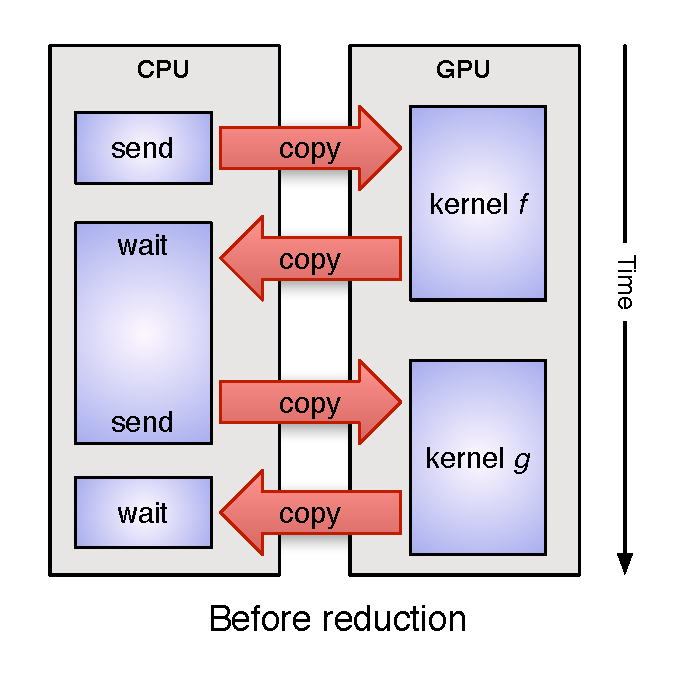
\includegraphics[width=2in]{images/reduction-before}&
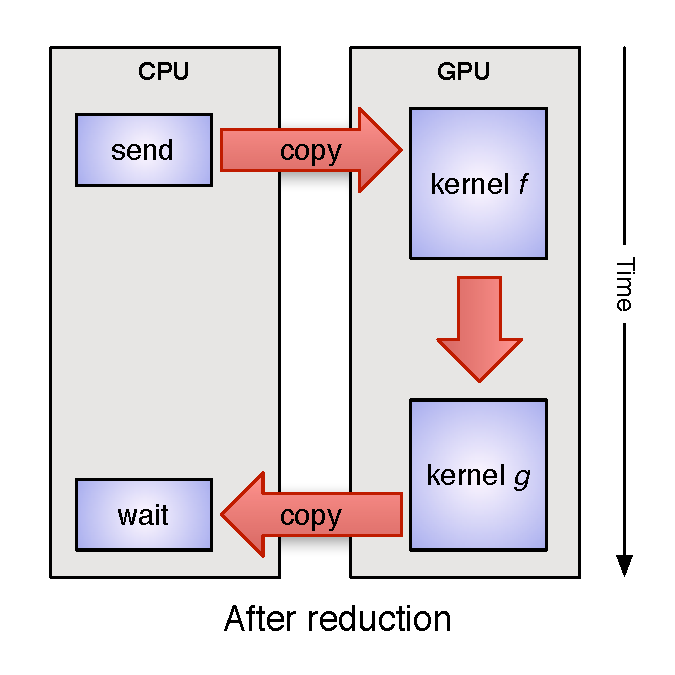
\includegraphics[width=2in]{images/reduction-after}\\
(a)&(b)\\
\end{tabular}
\caption{Elimination of redundant data movement. Part (a) depicts two GPU kernels called in sequence, unnecessarily copying data to and from the device. Part (b) shows the same program with the redundant copies removed.}
\label{basic-idea}
\end{figure}

Twig operates on data types instead of data. The input to a Twig program is a data type, and the output is a transformed data type along with some generated code that will perform the transformation on data in the target language. For this reason, Twig is restricted to operate only on types that can be represented in the target language, (e.g., for C, things like \texttt{int}, \texttt{float}, or \texttt{structs}). It can, however, augment the information about those types in order to make them more restrictive. For GPU programming, we exploit this capability with the addition of \emph{located types}.

Located types are a specific instance of the notion of \emph{augmented types}, in which the types provided by a base language are enhanced to carry important semantics that are implicit in the underlying language. For example, most languages support multi-dimensional arrays, but the ordering (column versus row major) is implicit. An augmented multi-dimensional array type would add this ordering as an explicit part of the type. In this way, the transition between representations would be explicit and clear in the code, instead of something implied by the base language itself.

\subsection{Located Types}
\label{sec:located-types}

For GPU programming, we augment standard data types with a  \emph{location}. The location information describes where the data is stored in memory, i.e., either in system memory or on the GPU.

For example, we can represent an array of \texttt{int}s on the CPU with the Twig type \texttt{array(int)}. The same type located on the GPU is \texttt{gpu(array(int))}. Any standard type may be wrapped inside the \texttt{gpu} type constructor.

Note that this location information is only used within Twig itself. In particular, it may or may not be reflected in the generated target type. If we are generating CUDA code, for example, the generated type for both \texttt{gpu(array(int))} and \texttt{array(int)} is simply a C pointer to \texttt{int} (i.e., \texttt{int *}). In this case, the location information is erased during the code generation phase. For other target languages or APIs that have a notion of location, the information could be preserved in the generated data types.

By augmenting basic data types with location information, we ensure that rules must be specific to the GPU in order to operate on GPU data. For example, a rule

\begin{verbatim}
[gpu(array(float)) -> gpu(array(int))]
\end{verbatim}

converts an ``array of floats'' data type to an ``array of integers'' type if and only if the type describes data located on the GPU. If the type describes data located elsewhere, its type must be ``converted'' (i.e., the data copied to the device) with a rule such as

\begin{verbatim}
[array(float) -> gpu(array(float))]
\end{verbatim}

This simple scheme enables automated reasoning about data motion.

It is important to understand that rules such as those given above describe transformations on \emph{data types}, not on the data themselves. It falls to the code that is generated as a consequence of successful application of these rules to perform the promised conversion on the actual data; this is described in Section~\ref{sec:code-gen}.

Located types could be used in more complex situations, as well. For example, they could be used track data moving between multiple GPU devices, with each device corresponding to a unique located type.
